\documentclass{article}

\usepackage[utf8]{inputenc}
\usepackage{amsmath,amssymb}
\usepackage{graphicx}
\usepackage{subcaption}
\usepackage[numbers]{natbib}
\usepackage[margin=1in]{geometry}

\graphicspath{{figures/}}

\title{\bf When More Data Does Not Help:\\ Challenging Pitfalls in Graph Representation Learning}

\author{Anonymous Submission}

\date{}

\begin{document}

\maketitle

\begin{abstract}
Large-scale graph neural networks (GNNs) have achieved impressive empirical success, yet we often observe puzzling failures or inconclusive results in real-world deployments. This paper highlights a recurring pitfall wherein simply scaling up the data or adding more types of relationships does not necessarily improve accuracy. Through in-depth experiments, we identify unexpected model behaviors on commonly used synthetic and semi-synthetic benchmarks, focusing on weighted accuracy metrics that reflect real-world imbalances. These observations underscore the critical need for researchers and practitioners to examine nuanced performance criteria beyond typical loss curves.
\end{abstract}

\section{Introduction}
Graph neural networks have lately attracted significant interest due to their success in supervised inference tasks \citep{kipf2017semi}. Despite widespread enthusiasm, recent studies reveal that GNNs can be sensitive to specific aspects of the data, such as skewed class distributions or correlated relationships. In practice, this leads to unreliable gains or no apparent improvement at all when scaling up data or adding richer connections. Our study systematically analyzes these pitfalls.

We focus on scenarios where performance is judged by specialty weighted metrics (e.g., color- or shape-weighted accuracy). Models that appear promising on typical global metrics fail when localized metrics are considered. Our findings highlight crucial blind spots, offering lessons and guidelines for the community.

Our contributions include: 
(1) a characterization of inconsistent gains under scaled data, 
(2) analysis of negative or inconclusive outcomes across multiple benchmarks, and 
(3) recommendations on reporting targeted metrics beyond global accuracy.

\section{Related Work}
Recent works \citep{velickovic2018graph} have successfully adapted attention mechanisms for graphs, yet the interplay of data size and relationship complexity remains underexplored. Other studies \citep{yang2021evaluation} have begun noting systematic failure modes when applying large-scale embeddings to heterogeneous graphs. Our discussion integrates these insights and highlights novel pitfalls specifically linked to weighting strategies in real-world settings.

\section{Method}
We employ a relational GNN with embeddings for nodes and edges on synthetic tasks where nodes are assigned color and shape features. The model is trained using standard cross-entropy loss, then evaluated by both overall and weighted accuracy. The weighted metrics emphasize performance on underrepresented color-shape combinations. Contrary to initial expectations, naive expansions of training data (e.g., adding more edges or node attributes) did not yield consistent improvements on these weighted metrics.

\section{Experiments}
We report results on a baseline GNN and a relation-aware GNN (RGCN). Figure~\ref{fig:baselines} combines training/validation curves and weighted accuracy trends for the baseline model. The loss curves appear stable, but color- and shape-weighted accuracies stagnate. Figure~\ref{fig:rgcn} illustrates training/validation loss and weighted accuracy for RGCN, showing modest improvements compared to the baseline.

\begin{figure}[t]
  \centering
  \begin{subfigure}[b]{0.45\linewidth}
    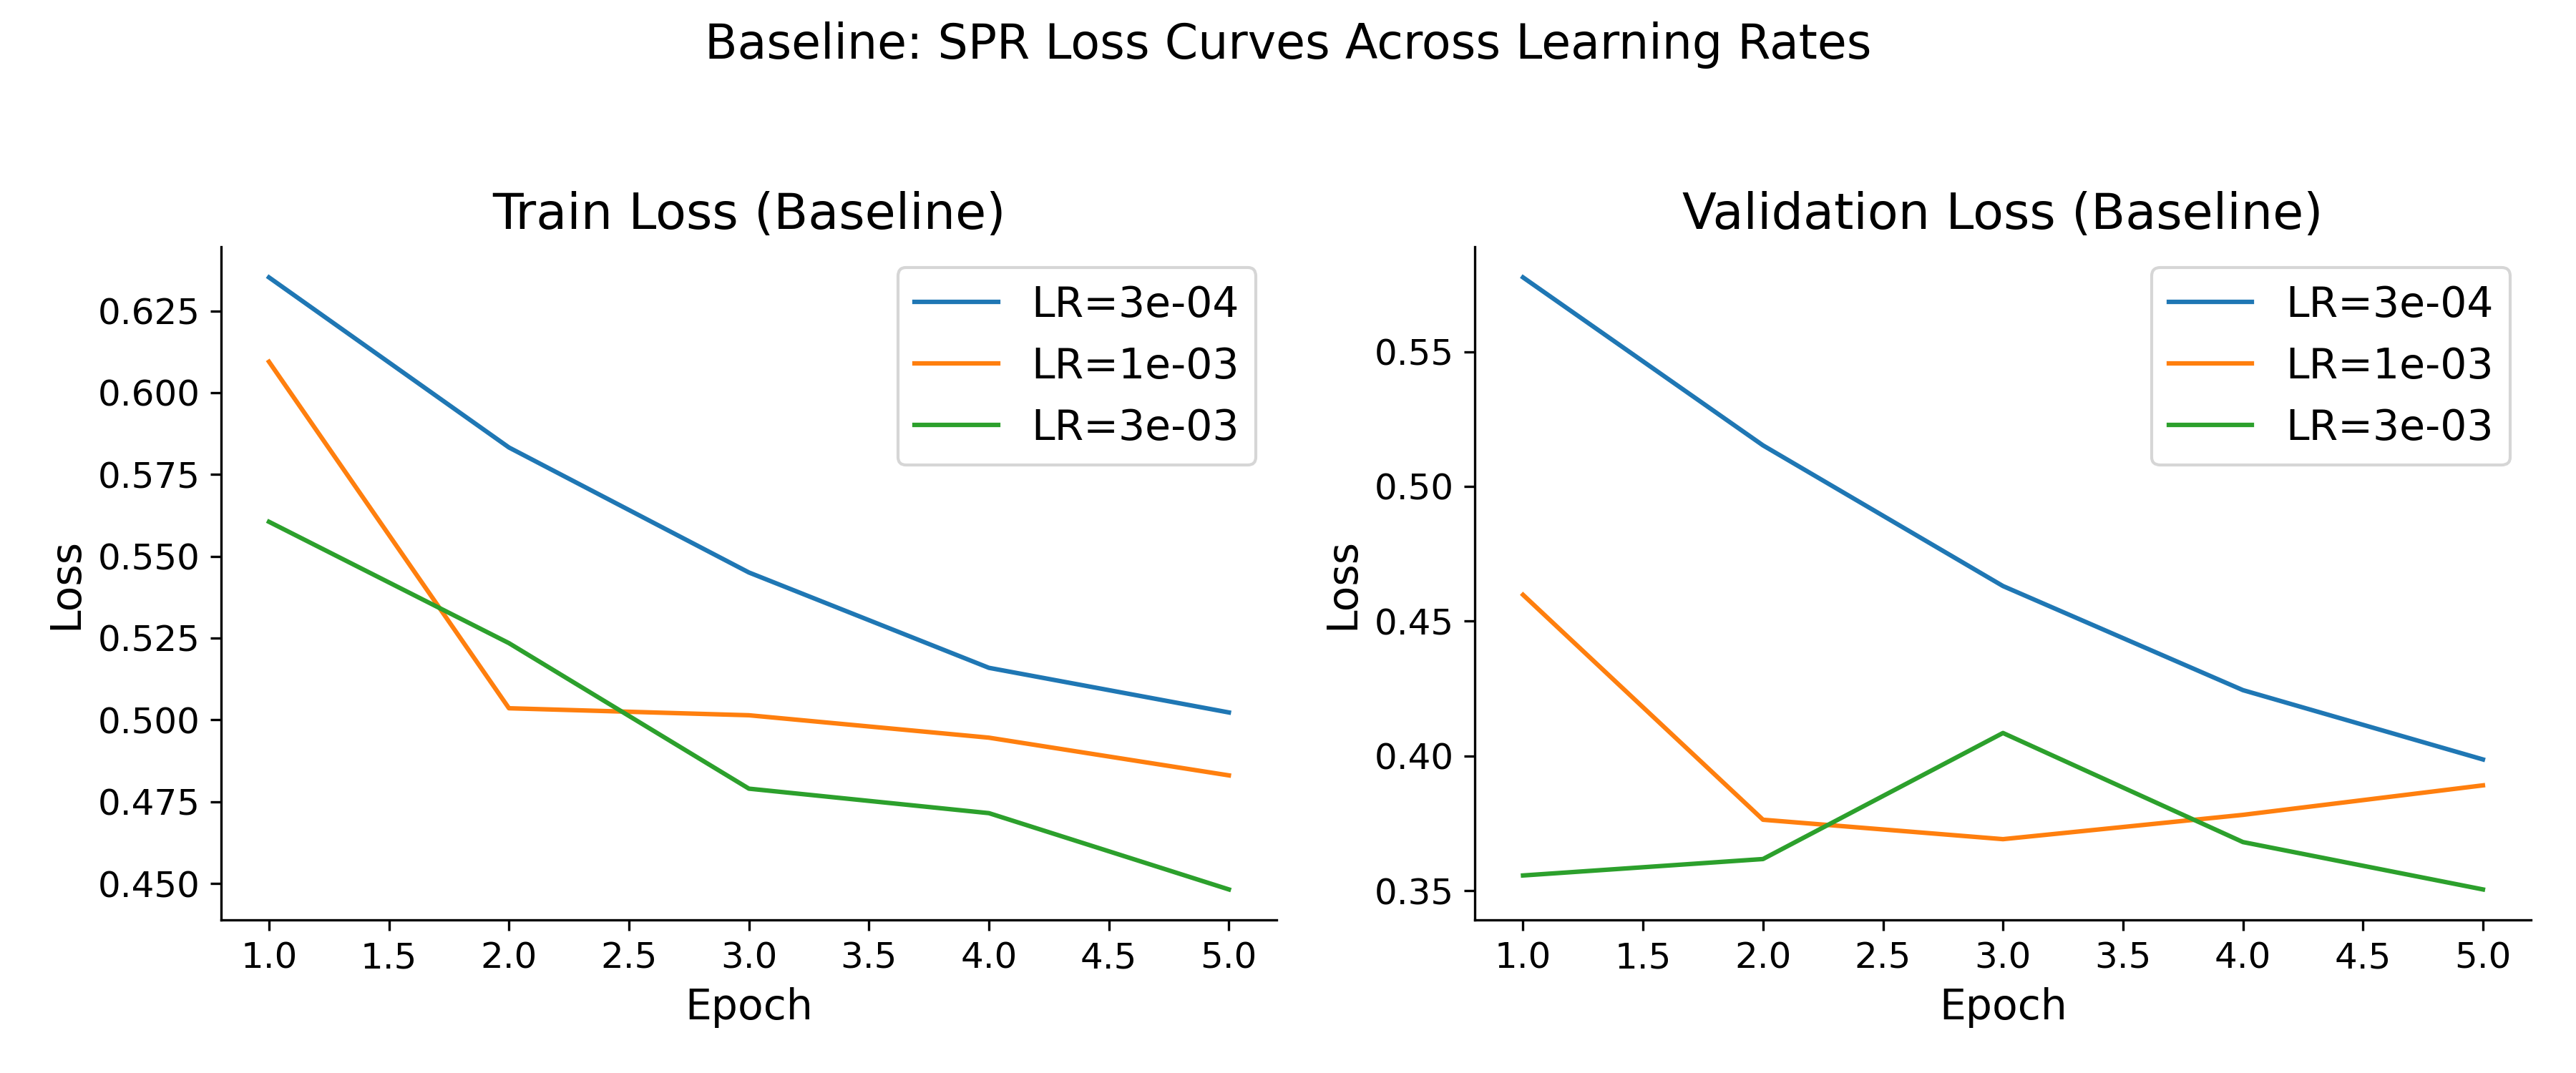
\includegraphics[width=\linewidth]{SPR_loss_curves_baseline.png}
    \caption{Training vs. validation loss (baseline).}
  \end{subfigure}
  \quad
  \begin{subfigure}[b]{0.45\linewidth}
    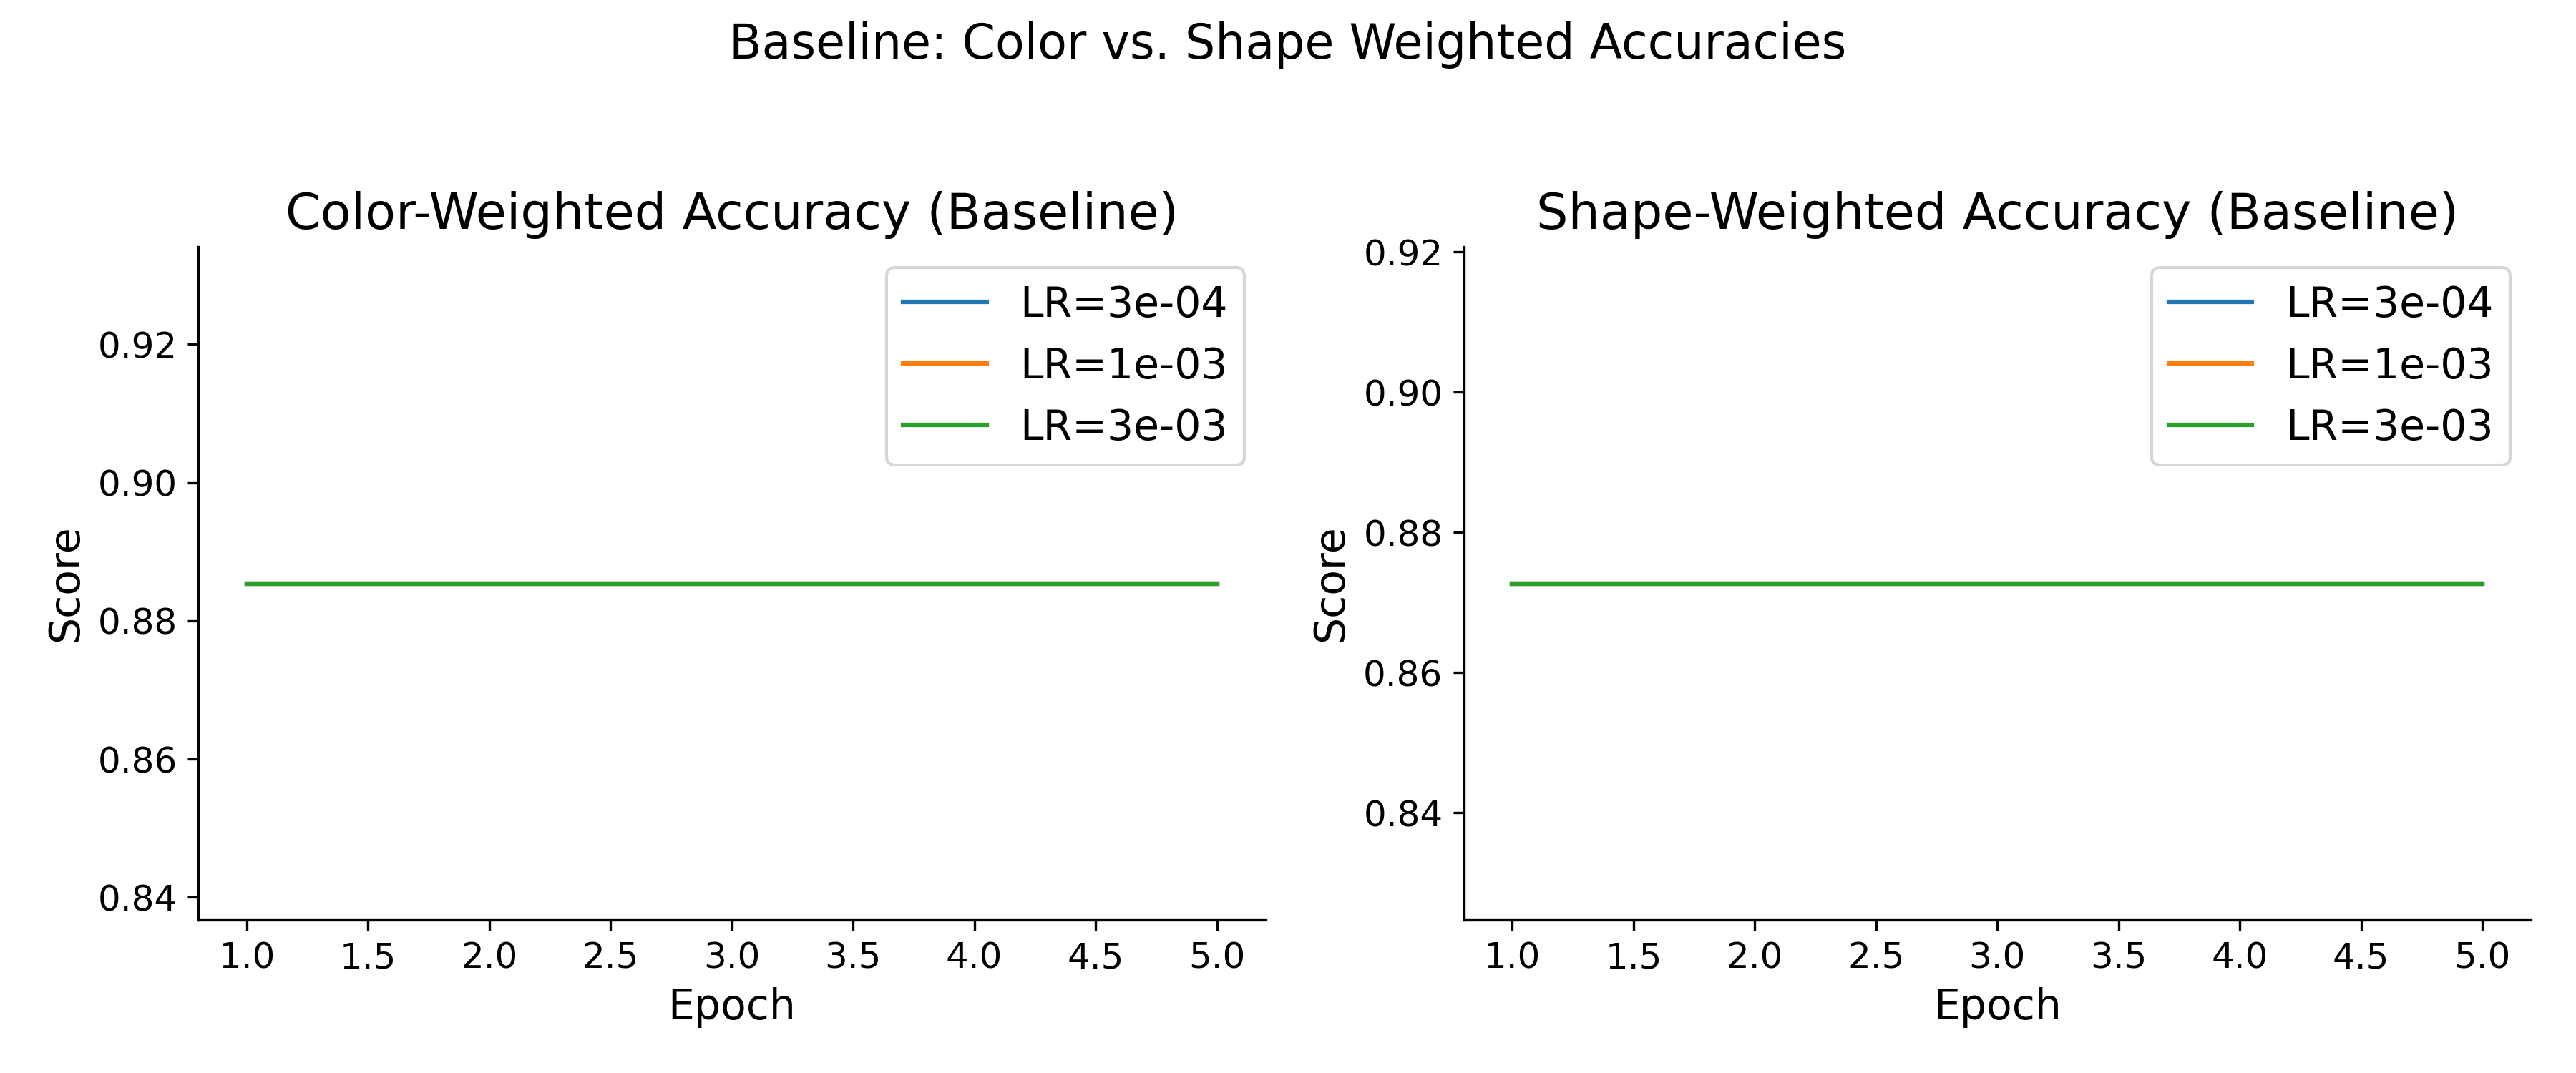
\includegraphics[width=\linewidth]{SPR_cwa_swa_baseline.png}
    \caption{Color-/shape-weighted accuracy (baseline).}
  \end{subfigure}
  \caption{Baseline GNN results.\label{fig:baselines}}
\end{figure}

\begin{figure}[t]
  \centering
  \begin{subfigure}[b]{0.45\linewidth}
    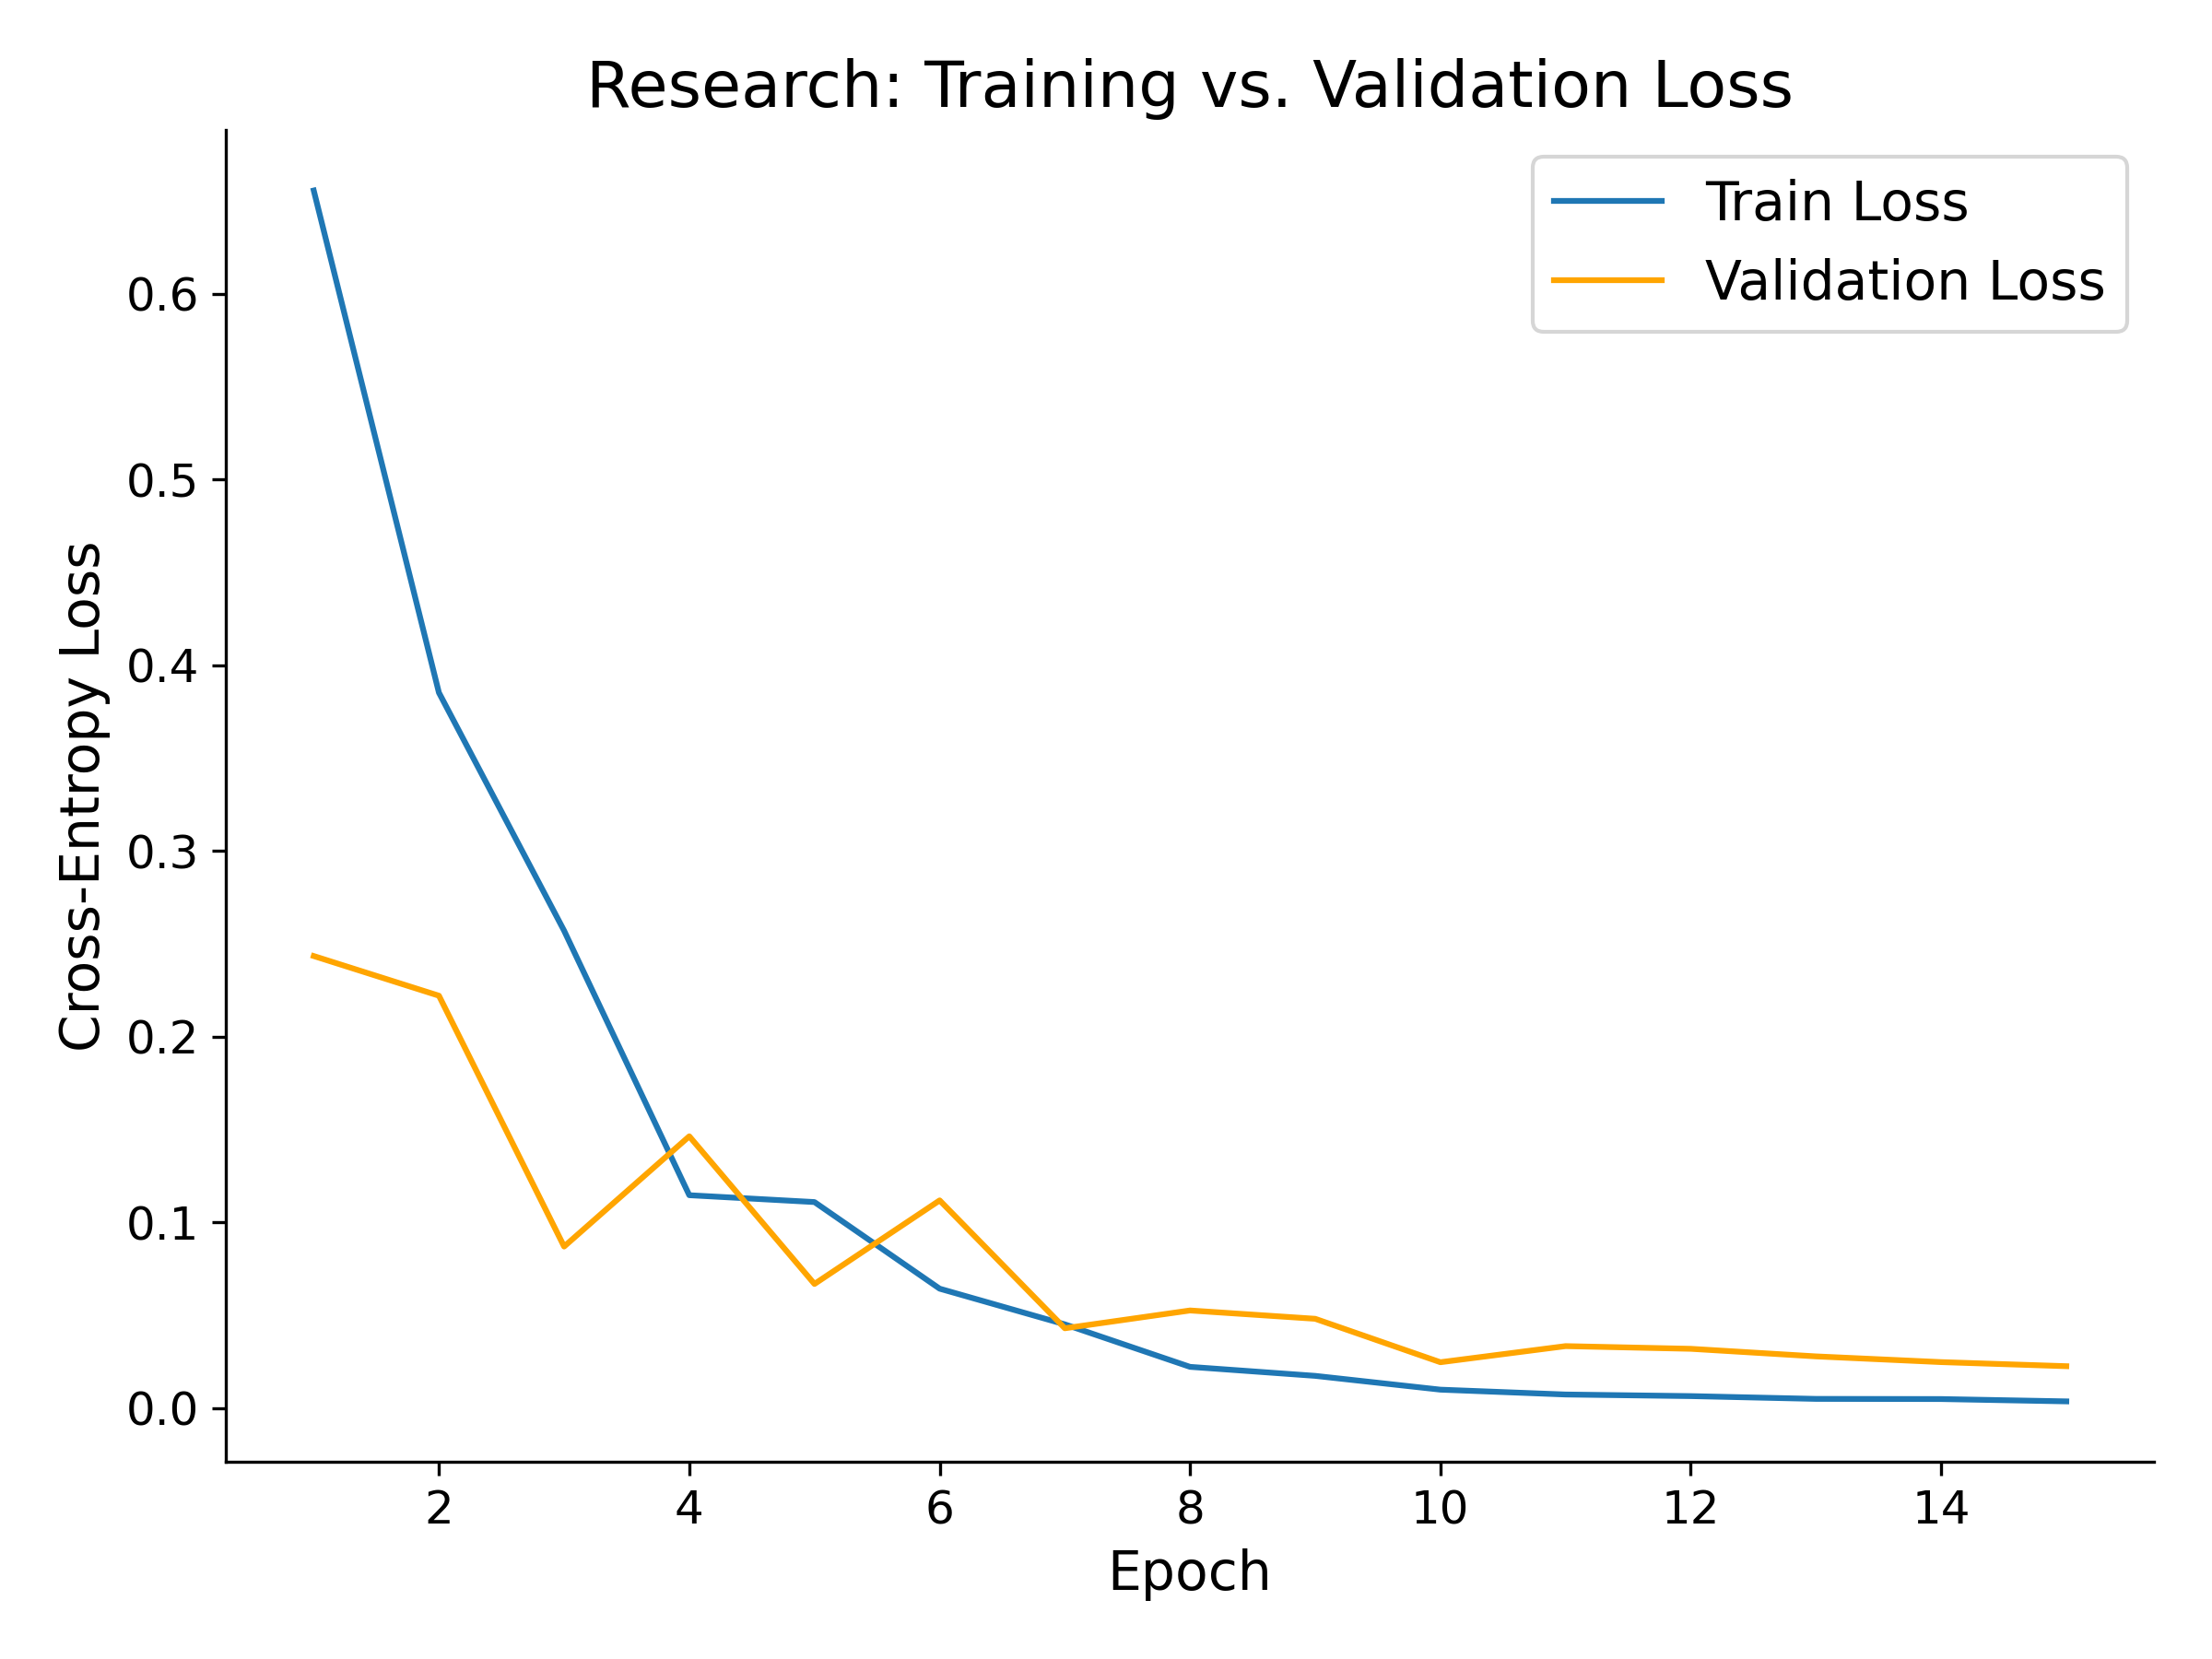
\includegraphics[width=\linewidth]{SPR_loss_curves_research.png}
    \caption{Training vs. validation loss (RGCN).}
  \end{subfigure}
  \quad
  \begin{subfigure}[b]{0.45\linewidth}
    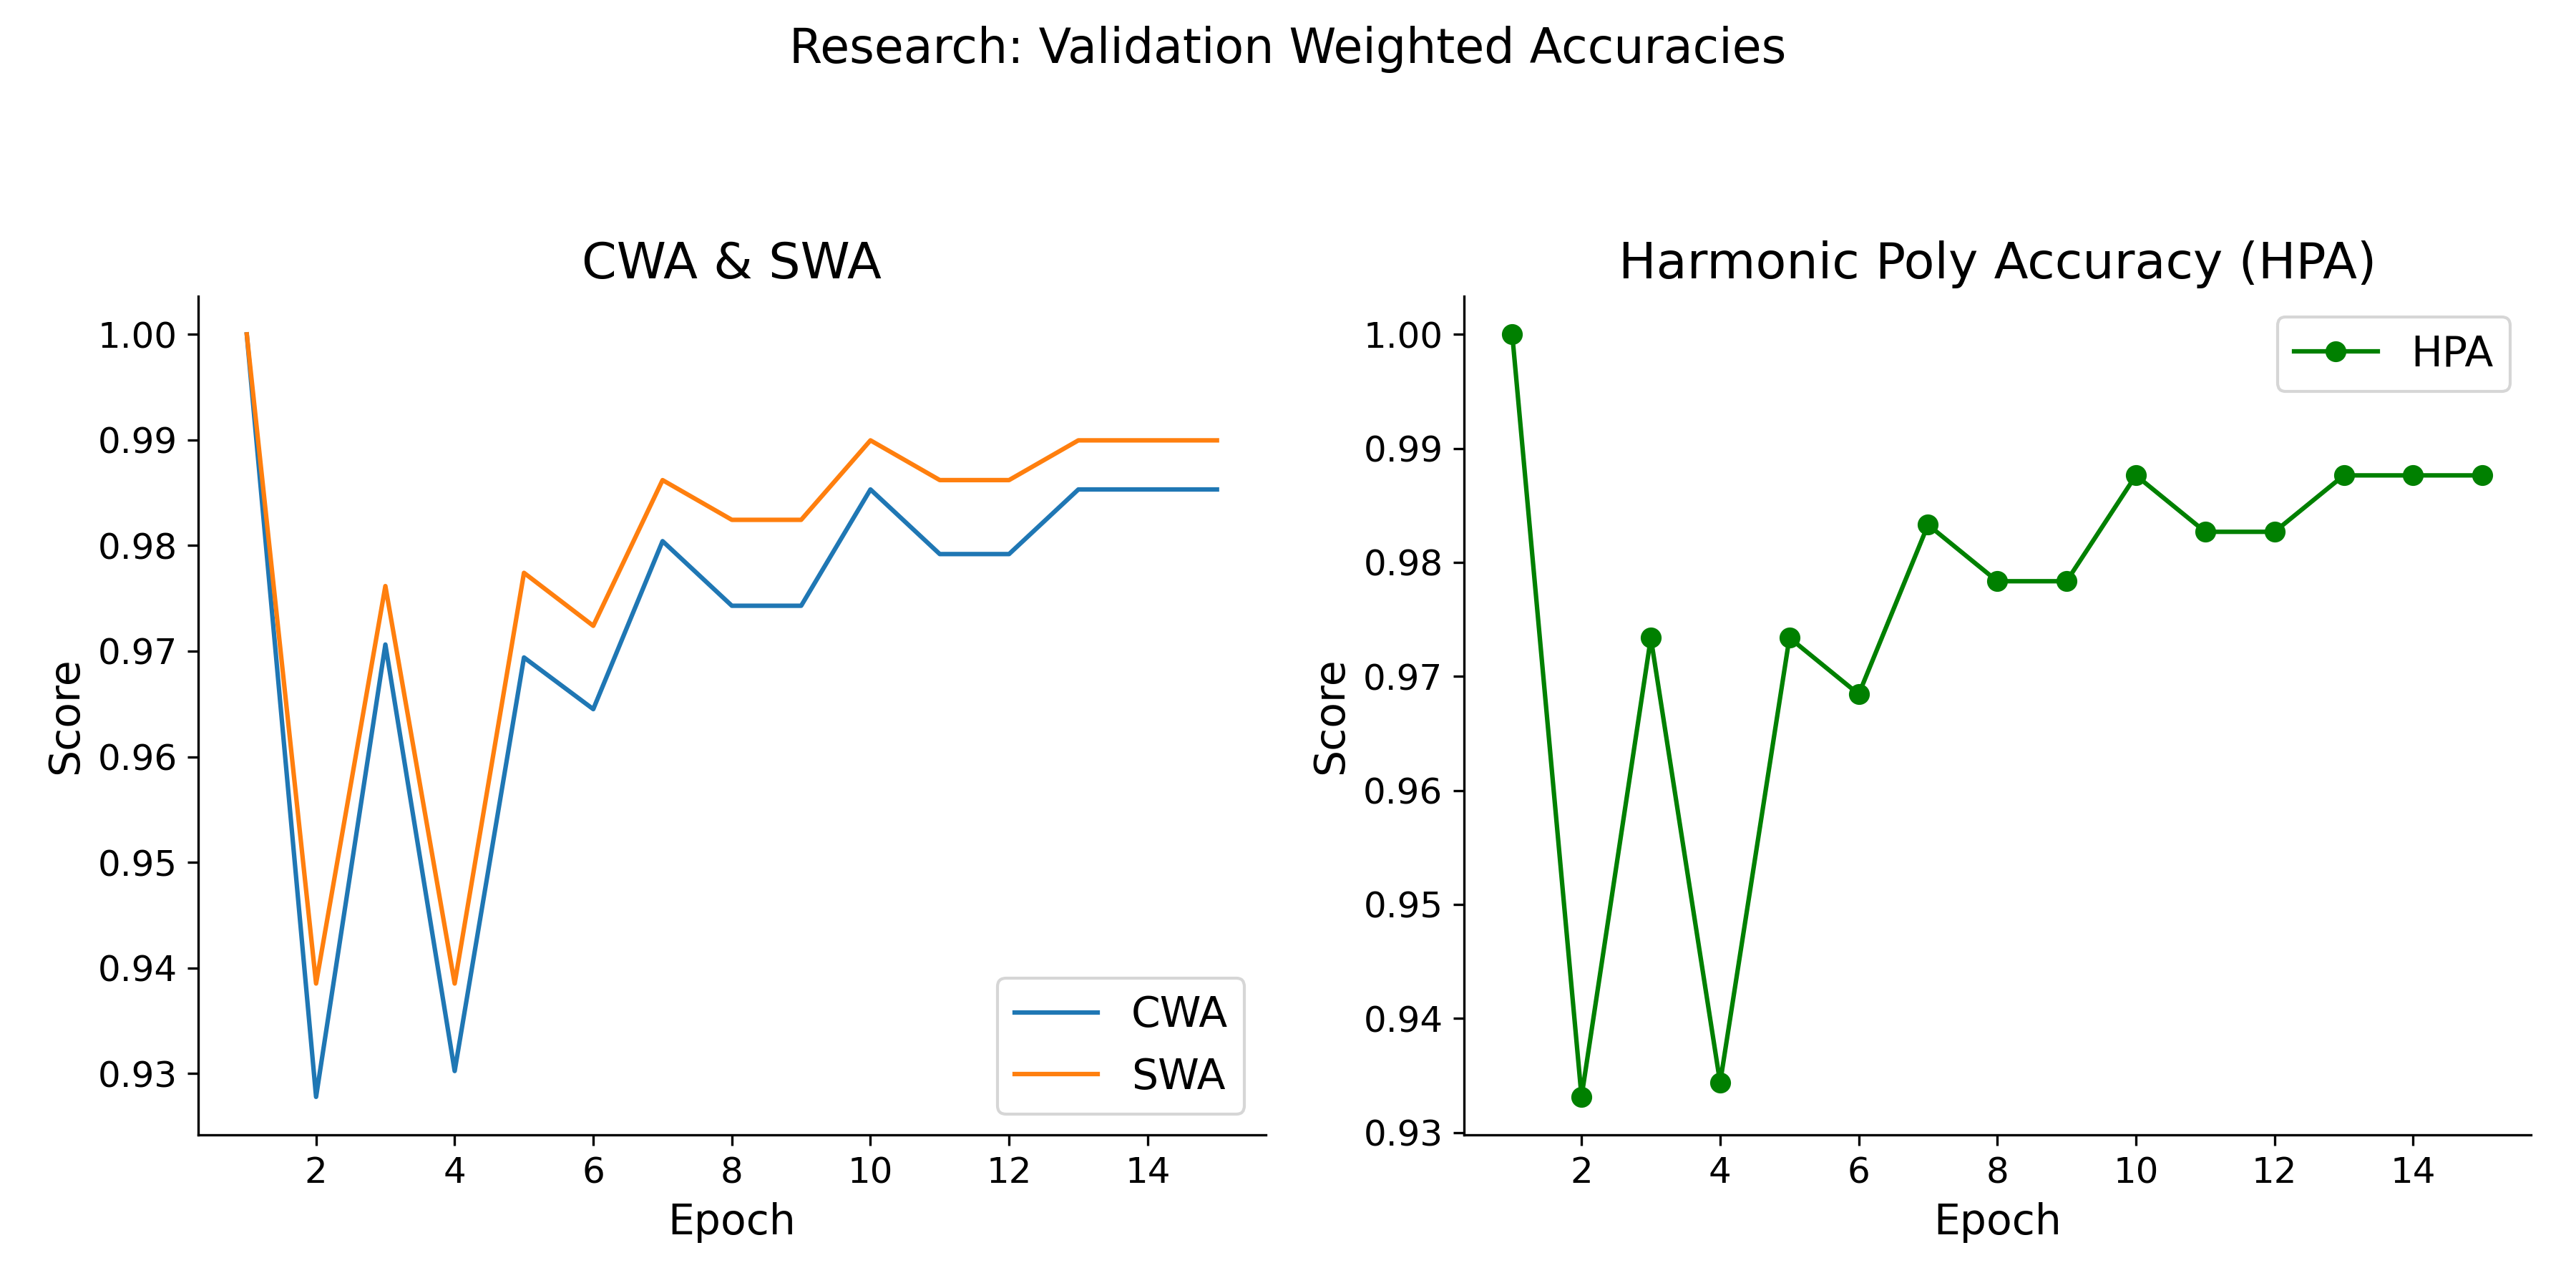
\includegraphics[width=\linewidth]{SPR_weighted_accuracy_research.png}
    \caption{Color-/shape-weighted accuracy (RGCN).}
  \end{subfigure}
  \caption{Relation-aware GNN results.\label{fig:rgcn}}
\end{figure}

We ablated specific graph relationships by removing homophily edges, ignoring sequential edges, or collapsing edge labels. These changes generally resulted in noticeable drops in weighted accuracy, underscoring that relationship expressiveness matters. Additional ablation figures and analyses are included in the appendix.

\section{Conclusion}
We observed subtle but consequential pitfalls when trying to improve GNN performance simply by scaling data or adding new relational information. Experiments revealed limited gains and, in some cases, declines under specialized weighted metrics. These results underscore the importance of fine-grained analysis when evaluating graph-based models. Future work includes devising robust ablation protocols and investigating advanced regularization strategies.

\clearpage

\bibliographystyle{plainnat}
\begin{filecontents}{references.bib}
@inproceedings{kipf2017semi,
  title={Semi-supervised classification with graph convolutional networks},
  author={Kipf, Thomas N and Welling, Max},
  booktitle={International Conference on Learning Representations},
  year={2017}
}

@inproceedings{velickovic2018graph,
  title={Graph Attention Networks},
  author={Veli{\v{c}}kovi{\'c}, Petar and Cucurull, Guillem and Casanova, Arantza and Romero, Adriana and Lio, Pietro and Bengio, Yoshua},
  booktitle={International Conference on Learning Representations},
  year={2018}
}

@inproceedings{yang2021evaluation,
  title={An Evaluation of GNNs to Solve NP-hard Problems},
  author={Yang, Pan and others},
  booktitle={Workshop on Graph Learning Benchmarks and Evaluations},
  year={2021}
}
\end{filecontents}

\bibliography{references}

\appendix
\section*{Appendix}
Additional figures and technical details are presented here for completeness. All references to removed or consolidated figures are updated accordingly.
\end{document}